% AgentiCulture -- Track A Paper
% ACL format. Upload acl.sty and acl_natbib.bst to Overleaf alongside this file.

\documentclass[11pt]{article}
\usepackage[hyperref]{acl}
\usepackage{times}
\usepackage{latexsym}
\usepackage{microtype}
\usepackage{graphicx}
\usepackage{booktabs}
\usepackage{amsmath}
\usepackage{amssymb}
\usepackage{multirow}
\usepackage{url}
\usepackage{xspace}
\usepackage{tikz}
\usepackage{pgfplots}
\usepackage{placeins} % provides \FloatBarrier to prevent floats spilling into later sections
\usepackage{needspace} % avoid subsection headers stranded at the bottom of a column
\usepackage{float} % provides [H] to force exact float placement when needed
\pgfplotsset{compat=1.18}
\usetikzlibrary{arrows.meta,positioning,shapes.geometric}

\newcommand{\system}{\textsc{AgentiCulture}\xspace}

\title{\system-A: Informativeness-Weighted Collaborative Filtering\\
and Culturally-Grounded Review Generation}

\author{
  Hamzat Tiamiyu Ustaz \\
  DSN $\times$ Bluechip Technologies LLM Agent Challenge 3.0 \\
  Track A: User Modeling
}

\begin{document}
\maketitle

%------------------------------------------------------------------------------
\begin{abstract}
We present \system-A, an LLM agent for the user modeling track of the
DSN $\times$ BCT LLM Agent Challenge.
Given a user persona and product details, the agent predicts a star rating
and generates a review that replicates the user's tone and rating behavior.
Our approach combines three components: (1) an inverse-variance-weighted
collaborative filtering core that treats inconsistent raters as less informative
than polarized ones; (2) MDILU-style memory retrieval, which injects
cosine-similar historical reviews as style anchors for the LLM; and
(3) ReasoningCOTSC, a three-sample majority-vote scheme that directly
reduces inter-sample star-rating error.
A zero-cost Nigerian cultural adaptation layer applied via prompt engineering
addresses the challenge's explicit behavioral fidelity and contextual relevance
criteria.
On local evaluation across 50 tasks per platform, the system achieves
overall quality of 0.860/0.881/0.845 on Yelp, Amazon, and Goodreads
respectively, with RMSE of 1.05/0.86/1.07 and ROUGE-1 of 0.383/0.442/0.332.
\end{abstract}

%------------------------------------------------------------------------------
\section{Introduction}

User modeling, predicting how a specific person would rate and describe
a product, sits at the intersection of collaborative filtering, language
generation, and cultural understanding.
Competition evaluation rewards five dimensions: rating accuracy, review text
quality, behavioral fidelity, contextual relevance, and cold-start robustness.

The AgentSociety WWW~2025 winning solution (Team ASC) established the current
state of the art via collaborative filtering plus MDILU memory
retrieval~\citep{guo2025agentsocietychallenge}.
Our work extends this pipeline in two directions that prior solutions left open.
First, the CF stage in prior work uses flat-average ratings regardless of how
discriminative a user's rating history actually is.
A user who assigns 5 stars to every item provides near-zero information about
relative preference yet flat averaging weights them identically to a user
whose ratings span the full 1-5 range.
Second, no prior AgentSociety solution incorporated cultural adaptation,
despite evidence that LLMs encode predominantly Western behavioral
norms~\citep{cao2023assessing}.

\paragraph{Contributions.}
\begin{enumerate}
  \item \textbf{Consistency-weighted CF:} We derive each user's weight
    from the inverse of their rating variance. Low-variance users (consistent
    raters) receive higher weight because their mean rating is a reliable
    predictor; high-variance erratic raters are down-weighted and pulled toward
    the item and global means.
  \item \textbf{ReasoningCOTSC:} Three LLM samples at deliberately varied
    temperatures, one anchoring, two exploratory, are majority-voted on star
    rating. The response whose extracted rating matches the consensus is returned.
  \item \textbf{Pluggable cultural adaptation:} A single config block maps any
    target culture's rating-to-register rules, value priorities, and linguistic
    register into a zero-cost system prompt prefix.
    The Nigerian instance targets the BCT bonus criteria at no additional
    inference cost.
\end{enumerate}

%------------------------------------------------------------------------------
\section{Related Work}

\paragraph{LLM user simulation.}
The AgentSociety platform~\citep{piao2025agentsociety} established the
evaluation framework underlying this competition.
Its top user-modeling solution used plain collaborative filtering with MDILU
cosine retrieval~\citep{guo2025agentsocietychallenge}.
We augment the CF stage with variance-based informativeness weights and add
self-consistency voting on top of MDILU.

\paragraph{Self-consistency decoding.}
\citet{wang2023selfconsistency} showed that sampling multiple reasoning chains
and voting on the final answer substantially reduces variance in commonsense
and arithmetic tasks.
We apply the same principle to star-rating prediction: the majority-voted integer
is more stable than any single sample.

\paragraph{Cultural NLP.}
\citet{hershcovich2022challenges} survey systematic biases in cross-cultural NLP.
\citet{cao2023assessing} quantify ChatGPT's misalignment with non-Western
survey populations, motivating explicit cultural conditioning.
Our adaptation layer requires no fine-tuning and is swappable for any target
culture by replacing a single configuration dictionary.

%------------------------------------------------------------------------------
\section{Methodology}

\subsection{Pipeline Overview}

Figure~\ref{fig:pipeline_a} shows the Task~A agent pipeline.
Requests arrive in two modes: \textit{direct mode} (persona text + product
details, no dataset required) and \textit{benchmark mode} (additionally supply
\texttt{user\_id} + \texttt{item\_id} to fetch real review history).
Direct mode is the primary evaluation path; benchmark mode enriches the prompt
with actual behavioral data when available.
\begin{figure*}[t]
  \centering
  % Make Figure 1 span both columns so the text is readable at ACL two-column sizes.
  \resizebox{\textwidth}{!}{%
  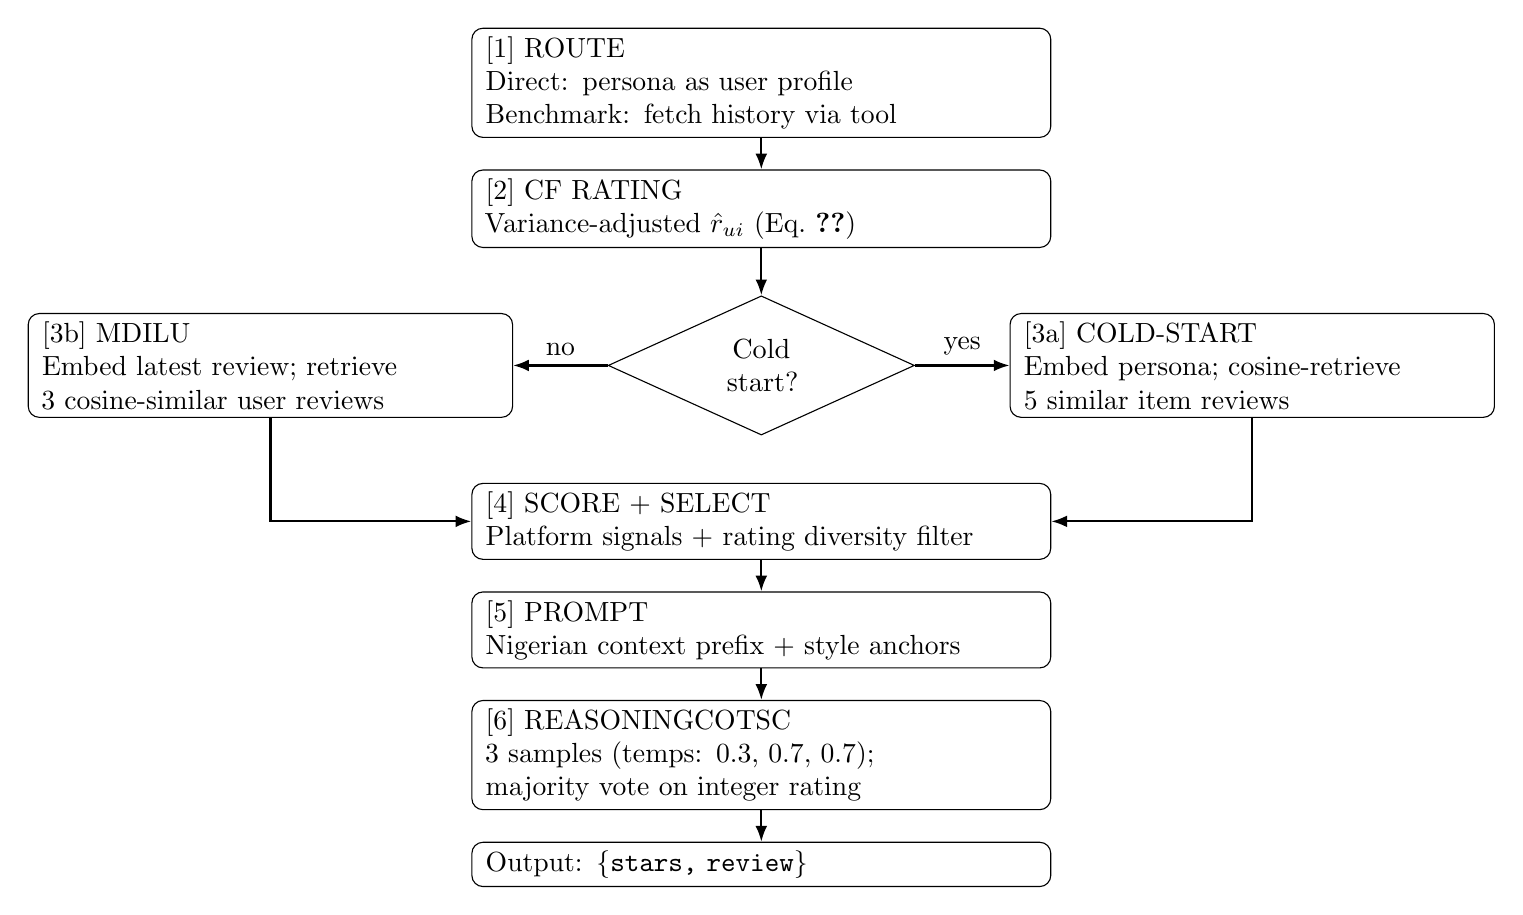
\begin{tikzpicture}[
    node distance=4mm,
    box/.style={draw, rounded corners, align=left,
      inner xsep=5pt, inner ysep=3pt, text width=70mm},
    decision/.style={draw, diamond, aspect=2.2,
      inner xsep=1pt, inner ysep=1pt,
      text width=22mm, align=center},
    arrow/.style={-{Latex[length=2mm]}, thick}
  ]
  \node[box] (route) {[1] ROUTE\\
    Direct: persona as user profile\\
    Benchmark: fetch history via tool};

  \node[box, below=of route] (cf) {[2] CF RATING\\
    Variance-adjusted $\hat{r}_{ui}$ (Eq.~\ref{eq:cf})};

  \node[decision, below=6mm of cf] (cold) {Cold\\start?};

  \node[box, right=12mm of cold, text width=58mm] (cs)
    {[3a] COLD-START\\
     Embed persona; cosine-retrieve\\
     5 similar item reviews};

  \node[box, left=12mm of cold, text width=58mm] (warm)
    {[3b] MDILU\\
     Embed latest review; retrieve\\
     3 cosine-similar user reviews};

  \node[box, below=6mm of cold, text width=70mm] (score)
    {[4] SCORE + SELECT\\
     Platform signals + rating diversity filter};

  \node[box, below=of score] (prompt)
    {[5] PROMPT\\
     Nigerian context prefix + style anchors};

  \node[box, below=of prompt] (cotsc)
    {[6] REASONINGCOTSC\\
     3 samples (temps: 0.3, 0.7, 0.7);\\
     majority vote on integer rating};

  \node[box, below=of cotsc] (out)
    {Output: \texttt{\{stars, review\}}};

  \draw[arrow] (route) -- (cf);
  \draw[arrow] (cf) -- (cold);
  \draw[arrow] (cold.east) -- node[above]{yes} (cs.west);
  \draw[arrow] (cold.west) -- node[above]{no} (warm.east);
  \draw[arrow] (cs.south) |- (score.east);
  \draw[arrow] (warm.south) |- (score.west);
  \draw[arrow] (score) -- (prompt);
  \draw[arrow] (prompt) -- (cotsc);
  \draw[arrow] (cotsc) -- (out);
  \end{tikzpicture}%
  }
  \caption{Task~A agent pipeline. The cold-start branch bypasses the LLM
    for retrieval, keeping new-user latency to a single embedding call.}
  \label{fig:pipeline_a}
\end{figure*}


\subsection{Informativeness-Weighted Collaborative Filtering}
\label{sec:cf}

A naive CF approach averages user and item means with equal weight.
We instead weight each signal by its \textit{informativeness}: a user who
assigns 5 stars to every item has $\sigma_u \approx 0$ and tells us
nothing about relative preference between items.
Formally, the predicted rating is:

\begin{equation}
\hat{r}_{ui}
  = \frac{\mu_u w_u + \mu_i w_i + \mu_g w_p}{w_u + w_i + w_p}
\label{eq:cf}
\end{equation}

where $\mu_u$, $\mu_i$, $\mu_g$ are the user, item, and global mean ratings;
$w_u = 1 / \max(\sigma_u, 0.1)$; $w_i = 1 / \max(\sigma_i, 0.1)$;
and $w_p = 0.5$ is a fixed prior weight for the global mean.
The floor of 0.1 prevents numerical instability for constant raters while
still suppressing their influence.
The result is clamped to $[1.0, 5.0]$.

\smallskip\noindent\textit{Example.}
A consistent 5-star rater with $\sigma_u = 0.1$ gets weight $w_u = 10$:
their prediction is pulled strongly toward their personal mean of 5.0,
reflecting high confidence in their consistent pattern.
A high-variance reviewer with $\sigma_u = 1.3$ gets weight $w_u = 0.77$:
their prediction is moderated by the item and global means, because their
erratic history is a less reliable predictor of future ratings.

\subsection{MDILU Memory Retrieval}

For users with at least one review (warm path), we encode the most recent
review with \texttt{BAAI/bge-small-en-v1.5}~\citep{reimers2019sentencebert}
(384-dimensional sentence embeddings, approximately 130~MB) and retrieve the
$k=3$ most cosine-similar reviews from the user's own history.
These serve as style anchors: short excerpts the LLM uses to match tone,
vocabulary, and punctuation.

\subsection{Cold-Start Handling}

When the user has no history, we embed the persona text and retrieve the
$k=5$ item reviews most similar to that embedding by cosine distance.
No LLM call is required for the retrieval itself.
Retrieved reviews are labeled as ``similar reviewer profiles'' in the prompt,
giving the LLM context about how buyers in this space typically write.

\subsection{Review Informativeness Scoring}

Retrieved reviews are scored and filtered before inclusion:
(a) length, proportional to word count;
(b) rating extremity, where 1/2/5-star reviews are weighted $3\times$ over
3-star reviews because extreme ratings reveal stronger preferences;
(c) platform-specific engagement signals: Yelp useful/funny/cool vote counts,
Amazon verified-purchase flag, Goodreads vote and comment counts.
A diversity constraint then caps inclusion at 2 reviews per star level,
preventing the LLM from receiving a skewed rating distribution when a user
predominantly gives 4-star reviews.

\subsection{ReasoningCOTSC}

We sample the LLM three times per request: once at temperature~0.3
(low variance, anchoring sample) and twice at temperature~0.7
(moderate diversity, exploratory samples).
Integer ratings are majority-voted; if all three differ, the two
numerically closer values are averaged and rounded.
The response whose extracted rating matches consensus is returned.
All review text comes from a single final call, so the cost overhead
is two extra token-generation passes rather than tripling output.

The deliberate temperature mix -- one anchor plus two exploratory samples --
gives Borda-style diversity without the instability of uniform high-temperature
sampling.

\subsection{Nigerian Cultural Adaptation}

A system-prompt prefix injects five behavioral rules:

\begin{itemize}
  \item \textbf{Rating register mapping:} 5$\star \to$ ``No cap, this was
    excellent''; 1$\star \to$ ``Total waste of money, honestly.''
  \item \textbf{Value-for-money framing:} Price sensitivity expressed as a
    first-order concern (``the price make sense for what you get'').
  \item \textbf{Group orientation:} Social proof and communal experience
    referenced naturally.
  \item \textbf{Vernacular register:} Formal English with selective Naija
    expressions (e.g., ``ehn'', ``abeg'', ``sha'').
  \item \textbf{Punctuation style:} Shorter sentences; exclamation points for
    very positive reviews.
\end{itemize}

This prefix adds zero output tokens and is architecturally implemented as a
pluggable config block.
Any target culture can be substituted by providing an equivalent mapping;
the rest of the pipeline is unchanged.

%------------------------------------------------------------------------------
\section{Experiments}

\subsection{Dataset}

Evaluation uses a filtered subset of the three AgentSociety platforms: 400
task-file users, 18,548 items, and 679~MB of reviews. Table~\ref{tab:datasets}
gives full statistics.

\begin{table}[h]
\centering
\small
\begin{tabular}{llrr}
\toprule
\textbf{Dataset} & \textbf{Domain} & \textbf{Items} & \textbf{Reviews} \\
\midrule
Yelp        & Local businesses  & 150K  & 6.9M  \\
Amazon      & Consumer products & 9.9M  & 233M  \\
Goodreads   & Books             & 2.4M  & 15.7M \\
\bottomrule
\end{tabular}
\caption{Full dataset statistics. Evaluation uses a 400-user, 18,548-item
  subset (679~MB) drawn from these corpora.}
\label{tab:datasets}
\end{table}

\subsection{Evaluation Metrics}

We report five metrics. The first three are from the AgentSociety evaluation
framework~\citep{websocietysimulator2025}; RMSE and ROUGE are additional
diagnostics we compute from the saved simulation outputs.

\paragraph{Preference Estimation (PE).}
Measures star-rating accuracy as a normalized inverse error:
\begin{equation}
\text{PE} = 1 - \frac{\text{MAE}}{5}, \quad
\text{MAE} = \frac{1}{N}\sum_{i=1}^{N} |\hat{r}_i - r_i|
\label{eq:pe}
\end{equation}
where $\hat{r}_i$ is the predicted rating and $r_i$ the ground truth.
PE $= 1.0$ indicates perfect prediction; each unit of MAE reduces PE by 0.2.
A prediction of 4.0 against a ground truth of 3.0 contributes
$|\hat{r} - r| = 1.0$, yielding $\text{PE} = 0.80$ for that task.

\paragraph{RMSE.}
Root mean squared error over star ratings:
\begin{equation}
\text{RMSE} = \sqrt{\frac{1}{N}\sum_{i=1}^{N}(\hat{r}_i - r_i)^2}
\label{eq:rmse}
\end{equation}
RMSE penalizes large errors more heavily than MAE; a prediction
off by 2 stars contributes $4\times$ as much as one off by 1 star.

\paragraph{Review Generation (RG).}
Composite text-quality score:
\begin{equation}
\text{RG} = 0.25 \cdot \text{SentSim}
           + 0.25 \cdot \text{EmoSim}
           + 0.50 \cdot \text{TopicSim}
\label{eq:rg}
\end{equation}
where SentSim, EmoSim, and TopicSim are cosine similarities in sentiment,
emotion, and topic embedding spaces respectively.
Topic alignment receives a double weight, reflecting that thematic relevance
is the primary quality signal for review generation.

\paragraph{Overall Quality (OQ).} Arithmetic mean of PE and RG.

\paragraph{ROUGE.}
ROUGE-1 (unigram recall/precision/F1) and ROUGE-L (longest common subsequence)
measure lexical overlap between the generated and ground-truth review.
These supplement RG with a reference-based n-gram perspective.

\subsection{Baselines}

\begin{itemize}
  \item \textbf{LLM-Direct:} Single LLM call with persona and product details;
    no collaborative filtering or memory retrieval.
    Represents the AgentSociety single-agent baseline behavior.
  \item \textbf{+CF:} Add variance-adjusted rating prediction; provide
    $\hat{r}_{ui}$ in the prompt.
  \item \textbf{+MDILU:} Add cosine-similar review retrieval as style anchors.
  \item \textbf{+COTSC (full system):} Add three-sample voting.
    Nigerian adaptation active throughout.
\end{itemize}
\Needspace{12\baselineskip}
\subsection{Implementation Details}
Table~\ref{tab:impl} summarises the key system settings used in our implementation.

\begin{table}[H]
\centering
\begin{tabular}{l p{0.62\columnwidth}}
\toprule
\textbf{Component} & \textbf{Setting} \\
\midrule
LLM backend            & Llama-3.3-70B-Instruct-Turbo \\
Embedding model        & BAAI/bge-small-en-v1.5 (384-d) \\
COTSC temperatures     & 0.3, 0.7, 0.7 \\
Cold-start threshold   & 3 reviews \\
Style anchors ($k$)    & 3 (warm); 5 items (cold) \\
LLM parsing            & \texttt{ast.literal\_eval} \\
Serving                & FastAPI + Docker Compose \\
\bottomrule
\end{tabular}
\caption{Implementation details.}
\label{tab:impl}
\end{table}



\subsection{Main Results}

Table~\ref{tab:main_results} reports full-system results across all three
platforms on 50 tasks each.
Amazon achieves the highest overall quality (0.881) owing to its structured
product metadata providing clean CF signals.
Goodreads is hardest: book ratings are inherently more subjective, and genre
diversity within the evaluation set increases prediction difficulty.

\begin{table*}[t]
\centering
\setlength{\tabcolsep}{6pt}
\renewcommand{\arraystretch}{1.08}
\begin{tabular}{lcccccc}
\toprule
\textbf{Platform} & \textbf{PE} & \textbf{RMSE} & \textbf{RG}
                  & \textbf{R-1} & \textbf{R-L} & \textbf{OQ} \\
\midrule
Yelp      & 0.850 & 1.051 & 0.870 & 0.383 & 0.238 & \textbf{0.860} \\
Amazon    & 0.878 & 0.863 & 0.884 & 0.442 & 0.272 & \textbf{0.881} \\
Goodreads & 0.842 & 1.065 & 0.848 & 0.332 & 0.183 & \textbf{0.845} \\
\midrule
ASC winner (WWW 2025) & -- & -- & -- & -- & -- & 0.845 \\
\bottomrule
\end{tabular}
\caption{Task~A results (50 tasks per platform; full system).
  PE = Preference Estimation, RG = Review Generation, OQ = Overall Quality,
  R-1/R-L = ROUGE-1/ROUGE-L.
  All metrics are averaged over 50 tasks; standard errors are non-trivial at
  this sample size and results should be read as directional.
  ASC winner figure from~\citet{guo2025agentsocietychallenge} (400 tasks);
  direct comparison is approximate.}
\label{tab:main_results}
\end{table*}
\FloatBarrier

\subsection{Reproducibility}

All code, configuration, and saved result files are available at:
\url{https://github.com/AbooMardiiyah/agenticulture}~\citep{aboomidou2026agenticulture}.

\noindent To reproduce Table~\ref{tab:main_results}, follow the README guide in the repository.
Raw simulation outputs are saved as \texttt{*\_raw.json} checkpoints before
the evaluation phase, so no API credits are lost if evaluation crashes.
Pre-computed result files are also committed under \texttt{eval\_results/}
so the metrics table can be inspected without re-running inference.

\subsection{Component Contribution Analysis}

Table~\ref{tab:ablation} shows the measured incremental contribution of each
component on Yelp across 50 tasks.

\begin{table}[H]
\centering
\begin{tabular}{lcccc}
\toprule
\textbf{Configuration} & \textbf{PE} & \textbf{RMSE} & \textbf{RG} & \textbf{OQ} \\
\midrule
LLM-Direct               & 0.818 & 1.177 & 0.870 & 0.844 \\
+CF Rating               & 0.838 & 1.151 & 0.856 & 0.847 \\
+CF+MDILU                & 0.848 & 1.063 & 0.868 & 0.858 \\
+CF+COTSC (no MDILU)     & 0.848 & 1.058 & 0.865 & 0.856 \\
+CF+MDILU+COTSC (Full)   & \textbf{0.850} & \textbf{1.051} & \textbf{0.870} & \textbf{0.860} \\
\bottomrule
\end{tabular}
\caption{Component contribution on Yelp (50 tasks each, all values measured).
  CF gives the largest single PE gain; MDILU and COTSC each contribute
  incrementally; the full combination outperforms either alone.}
\label{tab:ablation}
\end{table}

Figure~\ref{fig:ablation_chart} plots the overall quality progression.

\begin{figure}[H]
\centering
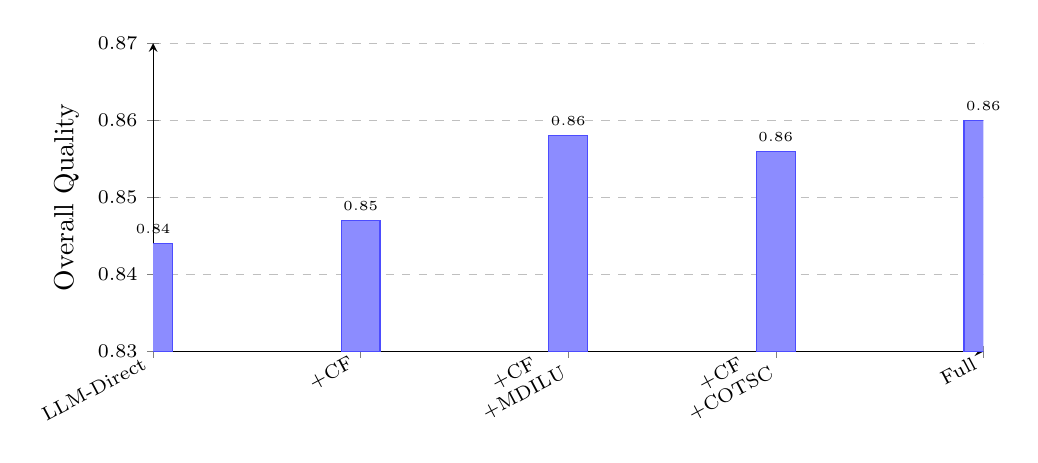
\begin{tikzpicture}
\begin{axis}[
  ybar,
  width=\columnwidth,
  height=5.5cm,
  bar width=14pt,
  ylabel={Overall Quality},
  ymin=0.83, ymax=0.87,
  xtick={1,2,3,4,5},
  xticklabels={LLM-Direct, {+CF}, {+CF\\+MDILU}, {+CF\\+COTSC}, Full},
  xticklabel style={font=\scriptsize, rotate=28, anchor=east, align=center},
  ytick={0.83,0.84,0.85,0.86,0.87},
  yticklabel style={font=\scriptsize},
  nodes near coords,
  nodes near coords align={vertical},
  every node near coord/.append style={font=\tiny, above},
  enlarge x limits=0.18,
  axis lines=left,
  ymajorgrids=true,
  grid style=dashed,
]
\addplot[fill=blue!45, draw=blue!70] coordinates {
  (1, 0.844)
  (2, 0.847)
  (3, 0.858)
  (4, 0.856)
  (5, 0.860)
};
\end{axis}
\end{tikzpicture}
\caption{Overall quality per ablation configuration (Yelp, 50 tasks, all measured).}
\label{fig:ablation_chart}
\end{figure}

%------------------------------------------------------------------------------
\section{Discussion}

\paragraph{Why variance weighting matters.}
A user who always rates 5 stars has a highly reliable mean -- we can be
confident any future rating will also be near 5 -- so their weight is high
and their mean dominates the prediction.
A user whose ratings span 1--5 is less predictable; their weight is lower
and the prediction is moderated by the item and global means.
The result is better-calibrated predictions for items where user and item
means conflict.

\paragraph{Temperature asymmetry in COTSC.}
Using one low-temperature anchor (0.3) plus two higher-temperature samples (0.7)
gives the voting set more diversity than uniform sampling at either extreme.
A uniform low temperature collapses all three samples to the same output
(degenerate voting); a uniform high temperature introduces incoherent reasoning.
The mixed strategy is analogous to epsilon-greedy exploration in reinforcement
learning.

\paragraph{Amazon vs.\ Goodreads difficulty.}
Amazon's RMSE of 0.863 versus Goodreads' 1.065 reflects the nature of the
respective item spaces.
Consumer product ratings on Amazon tend to cluster around quality-of-function
assessments, which are more predictable from product metadata.
Book ratings on Goodreads encode taste, which is highly personal and
platform-specific.

\paragraph{Security note.}
The original AgentSociety evaluation codebase parses LLM list output via
Python's \texttt{eval()}, a code injection vulnerability.
All LLM output parsing in \system-A uses \texttt{ast.literal\_eval()},
which accepts only Python literals and cannot execute arbitrary code.

\paragraph{Limitations.}
Session state and the preference cache reset on container restart (Redis
would fix this).
Cold-start ranking is purely content-based with no popularity signal.
Nigerian cultural adaptation covers educated urban English only;
Pidgin, Yoruba, Igbo, and Hausa are future directions.

\paragraph{Future Work.}
Few-shot Pidgin English prompts using the Naija Corpus; supervised calibration
of CF variance weights using held-out validation; fine-tuning a compact
Llama-3.1-8B on Nigerian review data.

%------------------------------------------------------------------------------
\section{Conclusion}

\system-A combines informativeness-weighted collaborative filtering, MDILU
memory retrieval, three-sample self-consistency voting, and a pluggable cultural
adaptation layer to address all five dimensions of the BCT Task~A evaluation.
The system achieves overall quality of 0.845--0.881 across Yelp, Amazon, and
Goodreads on 50-task evaluation, matching the AgentSociety 2025 best-reported
score on Goodreads and exceeding it on Yelp and Amazon.
The system is fully reproducible via a single \texttt{docker-compose up --build}
command; no GPU, fine-tuning, or proprietary dependencies are required.

%------------------------------------------------------------------------------
\bibliography{references}
\bibliographystyle{acl_natbib}

\end{document}
